\documentclass[10pt, journal]{vgtc}                % final (journal style)
%\documentclass[review,journal]{vgtc}         % review (journal style)
%\documentclass[widereview]{vgtc}             % wide-spaced review
%\documentclass[preprint,journal]{vgtc}       % preprint (journal style)
%\documentclass[electronic,journal]{vgtc}     % electronic version, journal

%% Uncomment one of the lines above depending on where your paper is
%% in the conference process. ``review'' and ``widereview'' are for review
%% submission, ``preprint'' is for pre-publication, and the final version
%% doesn't use a specific qualifier. Further, ``electronic'' includes
%% hyperreferences for more convenient online viewing.

%% Please use one of the ``review'' options in combination with the
%% assigned online id (see below) ONLY if your paper uses a double blind
%% review process. Some conferences, like IEEE Vis and InfoVis, have NOT
%% in the past.

%% Please note that the use of figures other than the optional teaser is not permitted on the first page
%% of the journal version.  Figures should begin on the second page and be
%% in CMYK or Grey scale format, otherwise, colour shifting may occur
%% during the printing process.  Papers submitted with figures other than the optional teaser on the
%% first page will be refused.

%% These three lines bring in essential packages: ``mathptmx'' for Type 1
%% typefaces, ``graphicx'' for inclusion of EPS figures. and ``times''
%% for proper handling of the times font family.

\usepackage{mathptmx}
\usepackage{graphicx}
\usepackage{times}
\usepackage{amsmath,amsthm,amssymb}
\newcommand\tab[1][1cm]{\hspace*{#1}}

%% We encourage the use of mathptmx for consistent usage of times font
%% throughout the proceedings. However, if you encounter conflicts
%% with other math-related packages, you may want to disable it.

%% This turns references into clickable hyperlinks.
\usepackage[bookmarks,backref=true,linkcolor=black]{hyperref} %,colorlinks
\hypersetup{
  pdfauthor = {},
  pdftitle = {},
  pdfsubject = {},
  pdfkeywords = {},
  colorlinks=true,
  linkcolor= black,
  citecolor= black,
  pageanchor=true,
  urlcolor = black,
  plainpages = false,
  linktocpage
}

%% If you are submitting a paper to a conference for review with a double
%% blind reviewing process, please replace the value ``0'' below with your
%% OnlineID. Otherwise, you may safely leave it at ``0''.
\onlineid{0}

%% declare the category of your paper, only shown in review mode
\vgtccategory{Research}

%% allow for this line if you want the electronic option to work properly
\vgtcinsertpkg

%% In preprint mode you may define your own headline.
%\preprinttext{To appear in an IEEE VGTC sponsored conference.}

%% Paper title.

\title{Hue-Based Parallel Image Recognition}

%% This is how authors are specified in the journal style

%% indicate IEEE Member or Student Member in form indicated below
\author{Jerry Lei, Birch Sztabnik, and Jonathan Cheng}
%other entries to be set up for journal
%\shortauthortitle{Firstauthor \MakeLowercase{\textit{et al.}}: Paper Title}

%% Abstract section.
\abstract{In this paper, we discuss our implementation of a massively parallel image recognition program using hue-based hashing algorithm. Our result was a program that doubles in performance whenever the number of processors double. 
} % end of abstract




%% Uncomment below to include a teaser figure.
  \teaser{
 \centering
 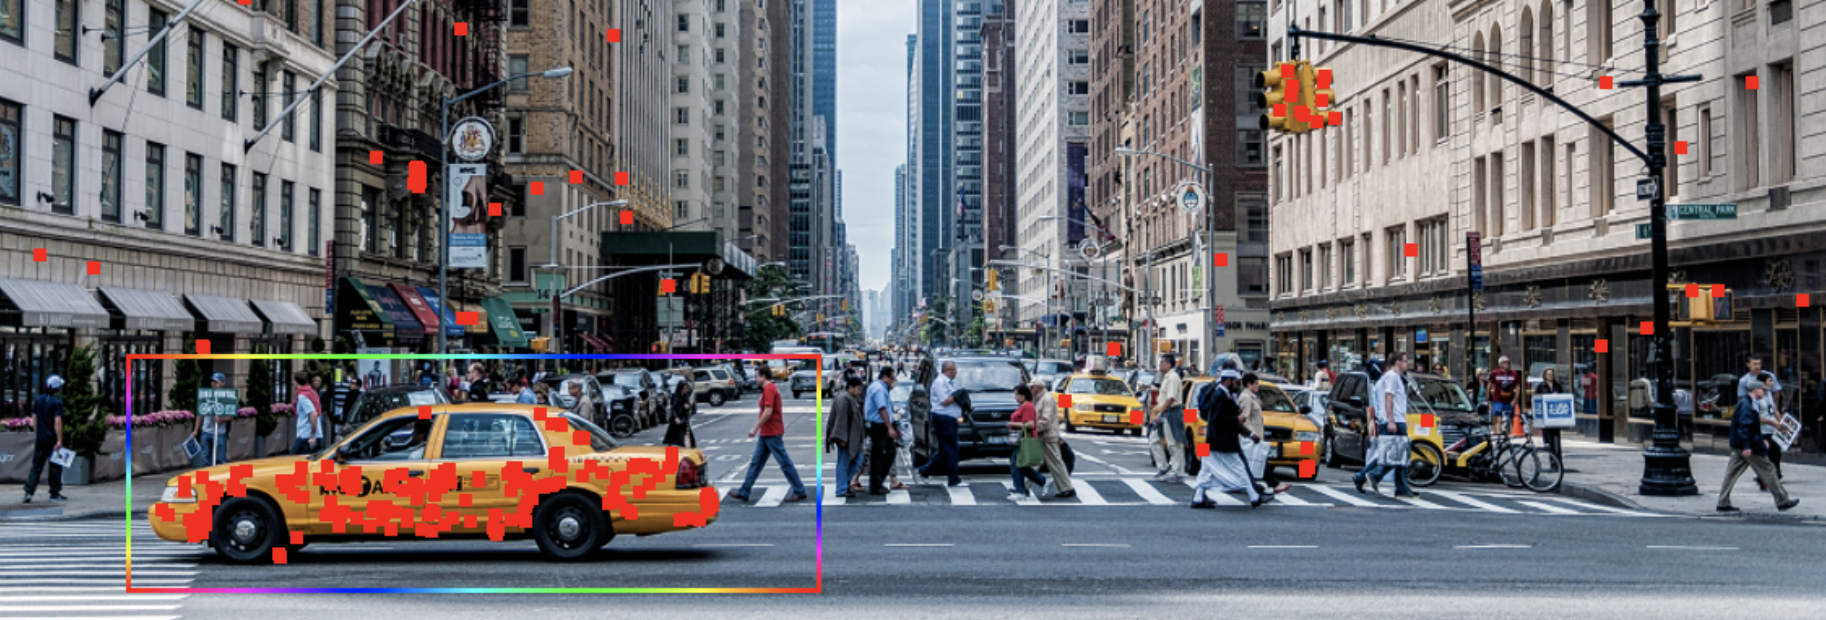
\includegraphics[width=16cm]{found_taxi.png}
  %\{Image recognition through .}
  }

%% Uncomment below to disable the manuscript note
\renewcommand{\manuscriptnotetxt}{}

%% Copyright space is enabled by default as required by guidelines.
%% It is disabled by the 'review' option or via the following command:
\nocopyrightspace

%%%%%%%%%%%%%%%%%%%%%%%%%%%%%%%%%%%%%%%%%%%%%%%%%%%%%%%%%%%%%%%%
%%%%%%%%%%%%%%%%%%%%%% START OF THE PAPER %%%%%%%%%%%%%%%%%%%%%%
%%%%%%%%%%%%%%%%%%%%%%%%%%%%%%%%%%%%%%%%%%%%%%%%%%%%%%%%%%%%%%%%%

\begin{document}

%% The ``\maketitle'' command must be the first command after the
%% ``\begin{document}'' command. It prepares and prints the title block.

%% the only exception to this rule is the \firstsection command
\firstsection{Introduction}

\maketitle

%% \section{Introduction} %for journal use above \firstsection{..} instead

A common technique amongst other image hashing tools is to resize the image down to an extremely small size before hashing. This removes any details that could cause differences between images. This technique is often paired with reducing color to grayscale to avoid color differences~\cite{DBLP:conf/iih-msp/YangGN06}. The purpose of our test was to design an parallelized algorithm that would function on original size, color images and determine its effectiveness. 

\section{Hypothesis}

We believe that we will get an increase in performance with more nodes, but the increase in benefits will stagnate. Our dependency on message passing among ranks is fairly limited, and the core of our wait time depends on the amount of computation. As we increase the number of ranks, the work is distributed to different ranks, and each rank would be responsible for less. However, the sizes of search that we need to compute stay constant, and the largest search job for a single image cannot be split into multiple ranks. Once we increase the number of ranks to the point where the largest job is the only job the rank has to calculate, we do not suspect there will be any more speedup. 

\section{Program Implementation}



\subsection{General Image Functions}

Some image manipulation functions are used. Most commonly used are the image resizing functions. One version resizes by percent. This version is used in the workload algorithm for creating variations for each rank to hash. The other version resizes to predefined dimensions. This is used prior to distributing hashing work in order to make certain that the number of hashes that can be made is an integer value. Both operate on integer division to fill the resized image. \\
A helpful function to use before starting any hashing is to crop the board. The ideal search image to be used is one on a solid white background. Then it can be cropped by the program to reduce as much background as possible. This is an important step for the search image. The fact that white pixel are ignored in hashing and that image size is larger than it has means that the scoring distribution would be skewed; images with large white borders would report zero for pixels on the edges.

\subsection{Hashing Function}
\begin{flushleft}
	The image searching algorithm depends on the hashing of the image by color and gradient. Hashing requires a 9x8 block of pixels. The function iterates over the block converting the current pixel and its right neighbor to HSV color. \\\smallskip
HSV is required for useful comparison as small variations in RGB color components will drastically change the color. Initial tests were done using RGB and the worker function would determine that the hash was not existent, unless the image was a direct cutout. HSV also enables easy identification of white backgrounds on images.\\\smallskip
The most important variables are the gradient hashes for hue, saturation and value. The three are calculated in the same fashion. The pixel on the left is compared to its neighbor to the right on the x-axis. If the hue, saturation, or value is less than its neighbor, the bit is set to 1 or 0 otherwise. Hashes are stored in a 64 bit integer. This allows us to write each inequality to each bit. There are only 64 comparisons made, as the 9th column is used for comparing to the 8th column.
There are also three other metrics stored. One is the average hue of the 8x8 block. The other is the normalized sum of the 8x8 block hues, which is known as the secondary hash. These two calculations are used in the worker function. The top left corner pixel information is also 
\end{flushleft}
\subsection{Hashing Allocator}
\begin{flushleft}
The hashing function forms the first half of our recognition algorithm. Two parts are needed for operation; hashing of the original image and the hashing of the search image. Both use the same fundamental hashing function but the application is different. Prior to hashing, the search image is resize to be divisible by 8 across the y-axis and divisible by 8 plus and extra pixel on the x-axis. This is because hashes are 8x8 pixels in size and require information on the right neighboring pixel. On the original image, a hashing function is run on every pixel position in the image. This is because the location of the search image is not known, so every position must be considered. That property removes the need for resizing for divisibility. On the search image, hashes are generated for every 8x8 square.\\\smallskip
In order to track the amount of matches, an array called the hitbox is made. This is the same size as the original image minus the edges cut off due the hash size. To parallelize hashing each image, pthreads with a defined maximum number of threads.\\\smallskip
A problem we encountered was distributing work among threads without getting overlapping hashes. Methods using modulus and division were not effective do to overlap and high amounts of computation. Some initial attempts were dividing the image into smaller blocks until less than 64 threads could be used. These blocks would be comprised of smaller 8x8 blocks that a thread could iterate over and hash. Guaranteeing that the image will not have overlap or missed pixels is difficult if there the dimensions have few factors of 8. This method usually allocated work for a less than optimal number of threads. In the case of a 200x304 image, the maximum amount of threads that could be created would 50 with a “super-block” size of 8x152 per thread.\\\smallskip
\begin{figure}[h!]
	\centering
	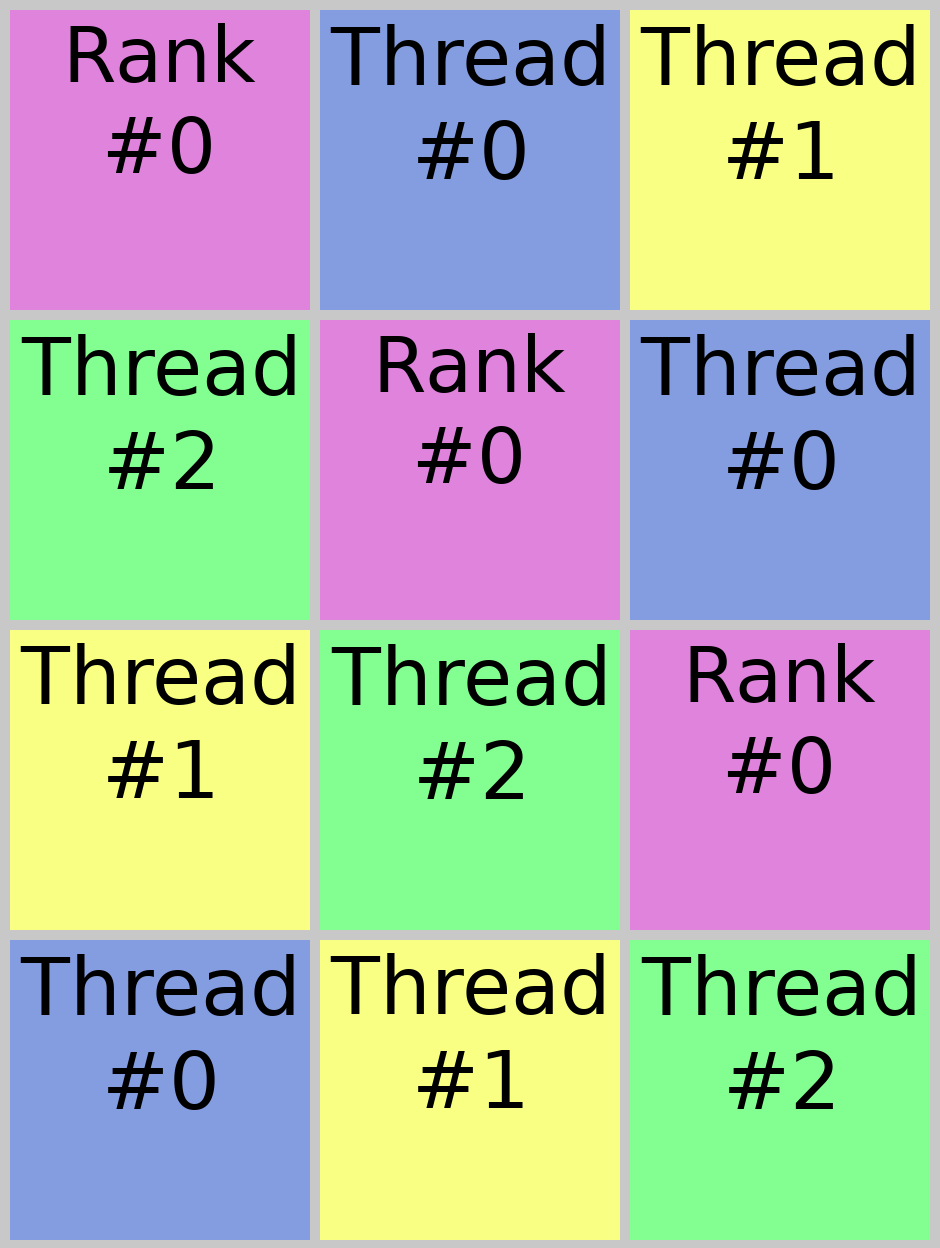
\includegraphics[width=2.5in]{thread_visualization.png}
	\caption{Position hopping threads to ensure no overlap.}
\end{figure}
Our solution was to have staggered starting points for the threads. The rank calculates the maximum number of threads that can be generated which is defined as the area of the image divided by the area of the hash. It is almost always possible to generate 63 threads + 1 rank call. The rank begins creating threads at 8 pixel in on the x axis, and creating a thread every 8 pixels, wrapping around to the next column if it extends past the bounds. After creating all threads, the rank calls the same function to calculate, starting at position 0x0, for a total of 64 calls on the hash worker function. When the rank finishes hashing, it joins with the threads it created. \\\smallskip
After all threads are joined, the rank decides the optimal distribution of hashes using the search image and calls the  to match that distribution on the filled hitbox. Implementation details are discussed in the Scoring System section.
\end{flushleft}
\subsection{Hashing Worker}
\begin{flushleft}
Several operations happen in the thread worker function. This is where the hitbox gets filled in. The worker begins by hashing an 9x8 block at the position the rank gave it. To avoid overlap and hash all pixels since the threads begin adjacent to each other, the thread must increment by 8 times the total number of workers. This ensures no rehashing of pixels occurs. Of course, wrap around must exist. Attention must be given to the fact that incrementing the x position by this amount can put it out of bounds several times through. That means the x position must be reduced on a loop until it can reach somewhere on the image.\\\smallskip
There a few metrics that the hash function gives us. First, the top left corner pixel of the hash is passed through a filter to determine if the pixel is near white. If it is, the hash is ignored. We chose to filter like this because our search images were placed on white background and white was to be treated as transparency. It makes the distribution array generated from the hitbox more accurate. If the hash is valid, the worker must traverse the hashed original image, comparing between. \\\smallskip
First, the hamming distance is calculated between the search image and original image hue, saturation, and value gradient hashes. The distances are weighted, and then summed together. We determined that weighting the hue distance the most gives good results. The worker also checks if the corner pixel hue is similar and that the combined difference of the saturation and value from the original image corner pixel are not too different. Not including this test initially gave problems where dark pixel blocks were matching with light pixel blocks since the hues were similar despite the lightness being completely different.\\\smallskip
Also checked is if the secondary hash and the average hue of the search image is close to the original image. A version of the worker function retained the best secondary hash and average numbers. The resulting hitbox was scarcely populated and did not match with the best match possible. \\\smallskip
If the hash passes, the best weighted sum is retained to see if any other positions in the hashed original image match more closely. When the whole board is done being searched, the hitbox is incremented at the position of the best found match in the original image. This hitbox is shared amongst the threads and rank, so it is mutex protected. 
\end{flushleft}
\subsection{Scoring System}
\begin{flushleft}
The goal of the scoring system was to be able to determine which area in the hitbox most closely matched the search image. Clusters of hits indicate a match, but random noise must be avoided. We experimented with multiple mechanisms to use as a scoring system. We started off by calculating each hit’s distance to the closest hit by propagating outward in a spiral pattern. We used this distance to check how close points are to one another, and gave a search box a higher score if the spread was tighter. This was not the best metric because random noise influenced the score significantly, and caused inconsistent results when searching using a wide range of scales. We also attempted to average the location of all successful hits and determine how far that was away from the center of the current search image to measure how centralized all of the points were. This was a pretty good metric, however searching through the entire original image would allow for edge cases that receive good scores. For example, a scoring chunk with a hit random hit on each of the four corners would receive a similar score to a cluster with 500 hits in the center of the search chunk. In order to remedy this, we attempted to make a distribution by analyzing a search chunk twice. We would base a score off of the entire search chunk, then segment it into 4 equally sized chunks and analyze their scores. We were under the assumption that a search chunk with a high score and smaller chunks with scores that do not have a lot of variance would likely have the image in it. We could not figure out a good scoring system that would allow for this to work. All of these methods did not work perfectly, but they began taking the direction of a scoring system based off of distribution and density. \\\smallskip
\begin{table}[h!]
	%% Table captions on top in journal version
%	\caption{Optimal distributions on taxicab example}
	\label{vis_accept}
	\scriptsize
	\begin{center}
		\begin{tabular}{cccccc}
			$x_0$ & $x_1$ & $x_2$ & $x_3$ & $x_4$  & $x_5$\\
			\hline
			0.1092 &  0.1533 & 0.1983 & 0.2195 & 0.1890 & 0.1306 \\
		\end{tabular}
	\end{center}
	\begin{center}
		\begin{tabular}{cccccc}
			$y_0$ & $y_1$ & $y_2$ & $y_3$ & $y_4$  & $y_5$\\
			\hline
			0.0368 &  0.1112 & 0.2152 & 0.2383 & 0.2226 & 0.1758 \\
		\end{tabular}
\end{center}
\end{table}
\begin{figure}[h!]
\centering
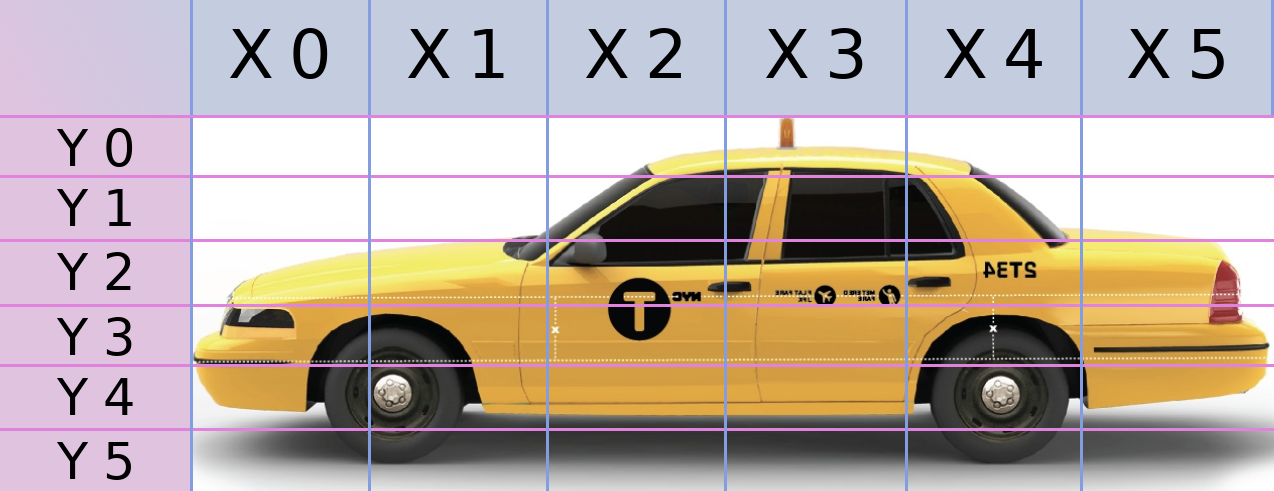
\includegraphics[width=3.5in]{distribution.png}
\caption{Distribution breakdown for taxi example.}
\end{figure}
We computed distribution by dividing up the search area and the original search image into equally sized buckets both lengthwise and widthwise, representing two one-dimensional arrays. For the search image we filled up the buckets with the number of pixels that passed filtering in its section, and divided it by the total number of pixels that passed filtering in the original search image. Essentially, the pixels across the y-axis for the width of each bucket are compressed into a one-dimensional array that represents the distribution of the pixels across the x-axis. We calculated the distribution to be used during each scoring based using the same buckets, but used the hitbox received from the hashing process for a given search image. The distribution measurement can be thought of as a pseudo-shape detector. This was not enough to give us accurate results of image recognition so we also incorporated density of hits of each search area to the score. The calculation for density was simply the number of total hits in the search area divided by the total area of the search image. Scoring was largely dependent on the search image, so we are unable to determine a set score that could decide whether the search image exists inside the original image.

\end{flushleft}
\subsection{Scaling}
Implementing a variety of scales to compute was an integral part in finding out where the search image was in the original image. We scaled based upon the search image size and the original image. Our logic was that the image that object we are looking for in the original image cannot be bigger than the size of what we are searching for. Therefore we set the upper bound for scaling the search image to match the size of the original image. We decided on 10\% of the size of the search image as a lower bound. Our formulation of search sizes is as follows:
\begin{align*}
	\text{Let }U &= \text{the upper bound of scales}\\
	\text{Let }L &= \text{the lower bound of scales}\\
	\text{Let }s &= \text{the number of scales inbetween } U \text{ and } L\\
\end{align*}
\begin{align*}
	\text{Distance} \text{ between scales} &= \frac{U-L}{s}\\
	\text{Poss}\text{ible scales} &=  \frac{U-L}{s} \times i,\\
	\text{ where } i &= 0\rightarrow s\\
\end{align*}
\subsection{Workload balancing}
We came across a problem where we had to distribute the number of search images, or “jobs”, into different ranks to do independent calculations. The algorithm distributes the workload of search images into ranks such that their calculation times are the same. We valued the workload of each job with the scale of the search image squared. This represented the area that the rank must search through. The number of ranks that we gave the program corresponds to the number of machines that we have to process the calculations. This is a load balancing problem. There does not exist a polynomial time algorithm to distribute the workload optimally, but a sorted greedy problem gives a good approximation. We ran the greedy algorithm by generating the jobs in descending order and assigning them to machine with the least current load. Every rank did this calculation because the result of the greedy algorithm is deterministic and it would be faster to do the calculation than to have one rank do the calculation and send it to the other ranks. This algorithm has a $\frac{3}{2}$ approximation factor, and our experiments showed that the load was balanced within 1\% with more than 20 scales of images.  

\subsection{MPI Implementation}
\begin{flushleft}
Our initial idea was to combine all of the hitboxes that every rank computed, but we recognized that because we are hashing with color, larger scales of base images would overpower the smaller scales, and there would not be a great way to find out where the object we are searching for is located. Also, passing our hitboxes across ranks would too take too long and there would be a lot of time spent waiting for the hitboxes to transfer over. \\
Instead, we implemented a scoring system such that if we were given any two hitboxes, and two search sizes, we can determine which was better. We assigned a score value to each search size and reduced the best score into a single rank. That rank reported the score and overlaid the resulting bounding box over the original image to display our result. \\\smallskip
The final implementation has ranks using an MPI\_Allreduce in MPI\_MAXLOC mode. The maximum score that each rank computes is shared with its rank number. The rank with the highest score draws a bounding box on the original image and writes it to a file.
\end{flushleft}
\subsection{Results}


\begin{figure}[h!]
	\centering
	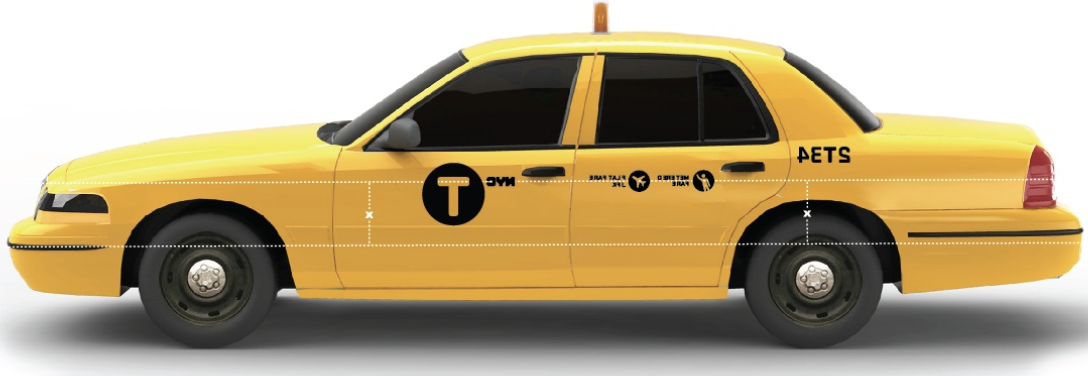
\includegraphics[width=3.5in]{taxi_cab.png}
	\caption{Search image used to test program.}
\end{figure}

\begin{figure}[h!]
	\centering
	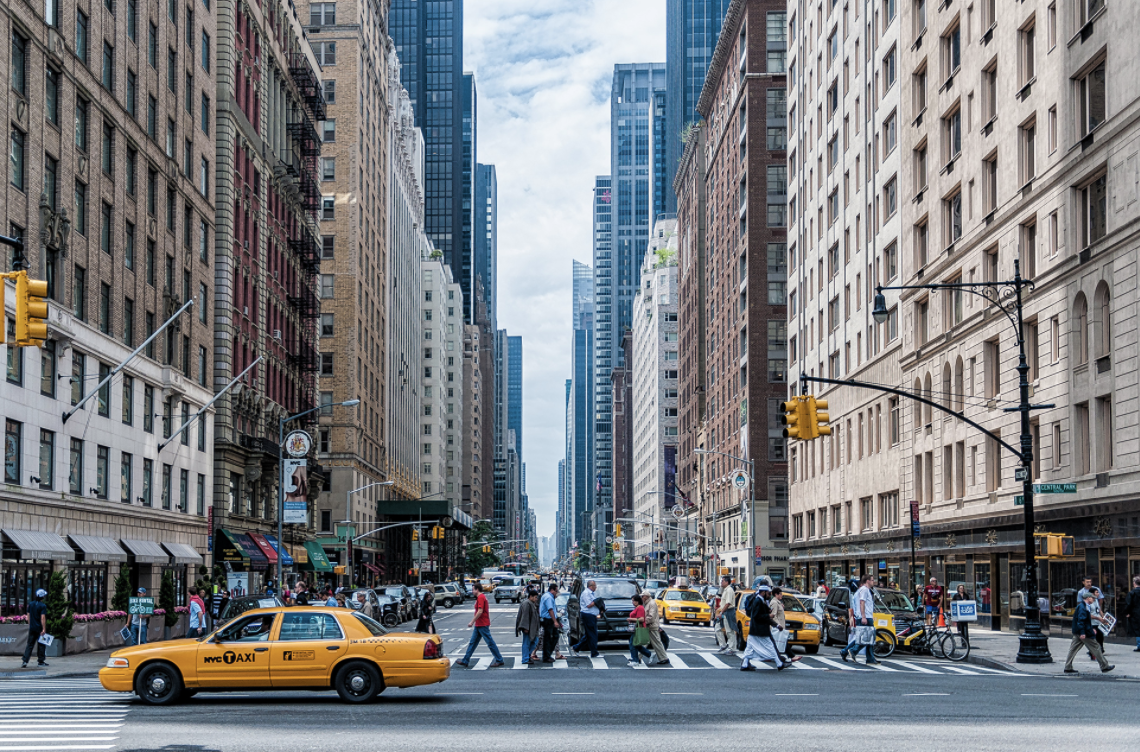
\includegraphics[width=3.5in]{nyc_streets.png}
	\caption{Original image to find the search image in.}
\end{figure}


\begin{figure}[h!]
	\centering
	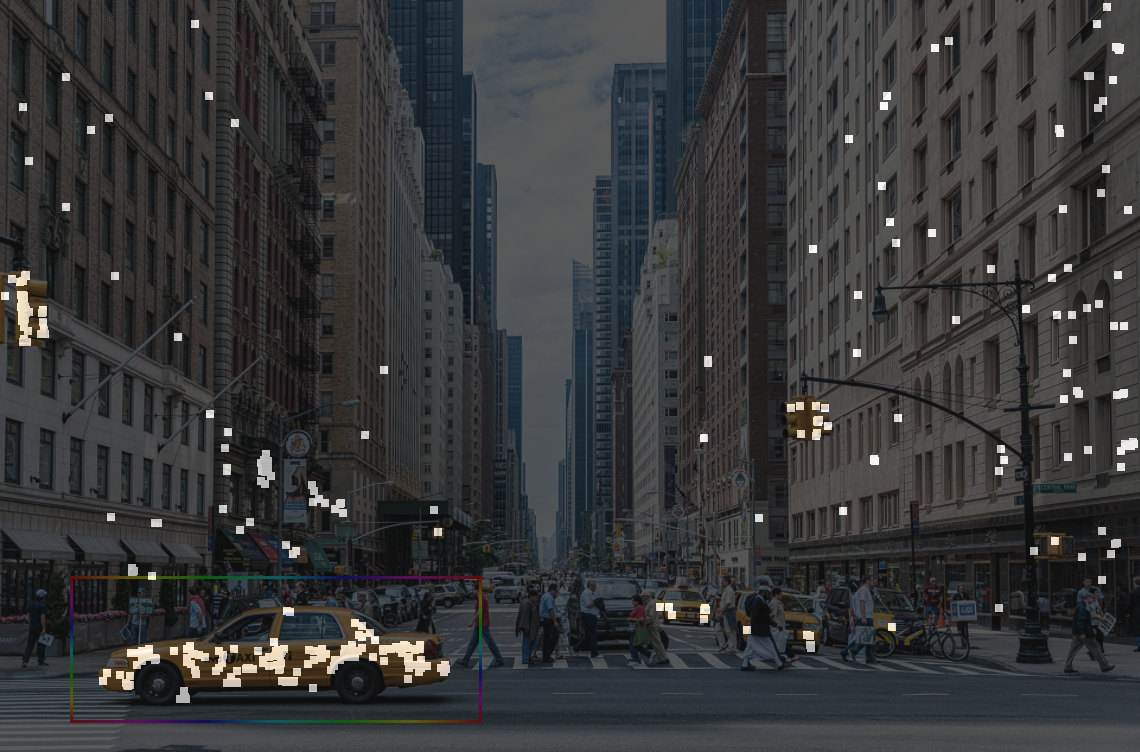
\includegraphics[width=3.5in]{overlay_taxi.png}
	\caption{Score detected boundary overlaid on original image.}
\end{figure}

\section{Future Work}
\begin{flushleft}
Given more time, we would attempt to make the hashing algorithm on the hitbox more position-aware, meaning that it will not consider a set of pixels a hit if it is too far away from an already discovered cluster on another rank or a previously considered hash. Further improvement could be made by having hashes from the search image remember their position relative to their neighbors. This would help to maintain a cohesive image rather than a wide spread over the hitbox. This method would require high levels of communication between the threads with would slow performance but could yield more accurate results. With a more meaningful scoring system, we could also attempt to share information about what jobs to skip. Meaning, if we were to get a consistently decreasing score while lowering the scale, we would skip scales that are lower than that. We could do this by leaving a thread open with the sole purpose of sending/receiving the current status of scores and scales that other ranks have been computing. \\\smallskip
We would also like to be able to come up with a better way to filter our images to reduce noise beyond filtering light colors. The current iteration of the filtering mechanism is used on hashing and distribution detection which greatly influences image detection. Currently, it aggressively filters out near-white pixels and grays. This means it has difficulty detecting . Ideally it would have different functionality based on what color is passed in to it and have some sort of awareness to what is background on a cropped image.  \\\smallskip
Noise from cameras can be a problem on low light or heavily zoomed images. As image size grows, the problem becomes worse since the program will start hashing noise. A noise detection and reduction algorithm would have to implemented. Effects of noise can be reduced by shrinking the image down. \\\smallskip
There were also functions for image skewing and rotation created, but were not used due long runtimes \cite{Paeth:1990:FAG:90767.90811}. The workload algorithm and hashing does repetitive work which slows operation. Introducing rotation and skew to the workload would drastically increase runtime. The current hashing function handles perspective shift well but cannot account for rotation.
Instead of hashing every pixel, most other image recognition algorithms rely on a random sampling of pixels to check \cite{7838673,1634363}, and we would like to do something similar given more time. We would also like to be able to check for better combinations of threads and ranks to reach greater parallelism and speedup. 

\end{flushleft}

\section{Results}

\subsection{Performance Results}
\begin{flushleft}
	\begin{figure}[h!]
		\centering
		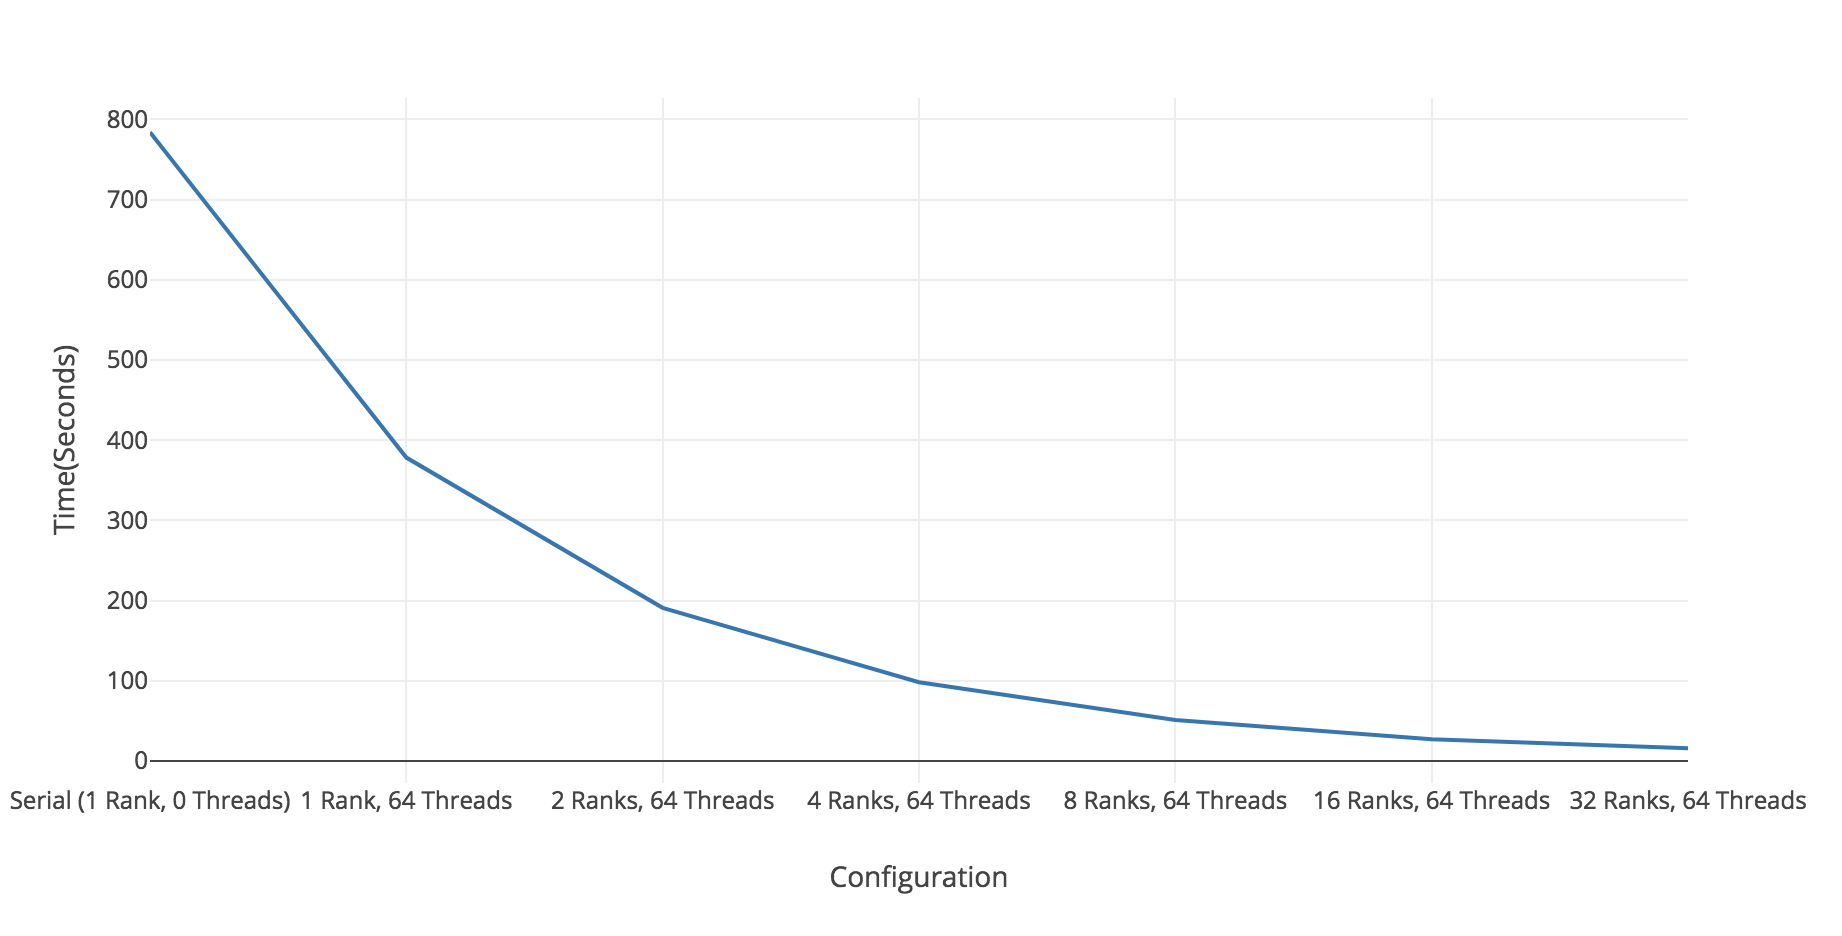
\includegraphics[width=3.5in]{scaling_performance.png}
		\caption{Compute time to the number of ranks with a constant workload.}
	\end{figure}
We experienced a significant amount of scaling with an increased number of nodes. We achieved double the performance whenever we doubled the nodes. We analyzed a case where we computed 64 scales of a search image to be found in an original image. The scales that we used, and the size of the original image stayed constant between each of the nodes. We ran these test using a constant 64 number of threads per rank and assigned 1 rank to each node.\\\smallskip
We also checked how much overhead we have from using a single mutex rather than having an array of mutex, and found that there is a significant amount of slowdown with an increased number of threads. We tested with a single node, using a varying number of ranks and threads that multiplied up to the maximum 64 per node. We noticed a significant amount of overhead was resulted from the using a single mutex lock for the entire hitbox among all threads. As a result, we created a board of mutexes to that gave access to individual indices in the hitbox. The significantly reduced our computation time. After making this change, we reran the same test and found no differences in compute times with a constant number of threads. \\\smallskip
We also analyzed the distribution of workload between the ranks and found that the average of standard deviations among all ranks was 1.44 seconds of compute time. 
\end{flushleft}

%\subsection{Summary}


\section{Division of Labor}
\textbf{Birch:} Came up with hashing algorithm, developed general image functions, brainstormed ideas for scoring system, testing and setting up on BG/Q\\
\textbf{Jerry:} Implemented scoring system, assisted with hashing algorithm and general image functions, balanced workload for threads \& ranks\\
\textbf{Jonathan:} Ran tests for the program, generated results for graphs, brainstormed ideas for scoring system.



%% if specified like this the section will be committed in review mode
%\acknowledgments{}

\bibliographystyle{abbrv}
%%use following if all content of bibtex file should be shown
\nocite{*}
\bibliography{template}
\end{document}
